\qrchapter{https://forgottenpillar.com/rsc/en-fp-chapter8}{The constructive criticism}


\qrchapter{https://forgottenpillar.com/rsc/en-fp-chapter8}{La crítica constructiva}


The first point of the \emcap{Fundamental Principles} answers the questions: who is God, what is His personality, and how do we understand His presence?


El primer punto de los \emcap{Principios Fundamentales} responde a las preguntas: ¿quién es Dios?, ¿cuál es su personalidad y cómo entendemos su presencia?


\others{I. That there is \textbf{one God}, \textbf{a personal, spiritual }\textbf{\underline{being}}, \textbf{the creator of all things}, omnipotent, omniscient, and eternal; infinite in wisdom, holiness, justice, goodness, truth, and mercy; unchangeable, and \textbf{everywhere present by his representative, the Holy Spirit}. Ps. 139:7.}[FP1889 147.2; 1889][https://egwwritings.org/read?panels=p931.6]


\others{I. Que hay \textbf{un solo Dios}, \textbf{un ser personal y espiritual}\textbf{\underline{,}} \textbf{creador de todas las cosas}, omnipotente, omnisciente y eterno; infinito en sabiduría, santidad, justicia, bondad, verdad y misericordia; inmutable y \textbf{presente en todas partes por medio de su representante, el Espíritu Santo}. Salmo 139:7.}[FP1889 147.2; 1889][https://egwwritings.org/read?panels=p931.6]


The one God, the Creator, is identified as the Father, because the second point of the \emcap{Fundamental Principles} states that Jesus Christ, the Son of the Eternal Father, is the one by whom God created all things\footnote{\href{https://egwwritings.org/?ref=en_FP1889.147.3&para=931.7}{FP1889 147.3; 1889}}. The \emcap{personality of God} is expressed in the term “\textit{personal spiritual being}”. We will soon see that this term denotes that the Father has a material body, a physical manifestation. Thus, in His personality, He is present only where He dwells physically. But, His presence is not constrained to His personality because He is \others{everywhere present by his representative, the Holy Spirit}. During our past history, this understanding and reasoning of the \emcap{personality of God}, as expressed in the first point of the \emcap{Fundamental Principles}, received constructive criticism; by “constructive criticism” we refer to the criticism supported by the Bible.


El único Dios, el Creador, se identifica como el Padre, porque el segundo punto de los \emcap{Principios Fundamentales} afirma que Jesucristo, el Hijo del Padre Eterno, es aquel por quien Dios creó todas las cosas\footnote{\href{https://egwwritings.org/?ref=en_FP1889.147.3&para=931.7}{FP1889 147.3; 1889}}. La \emcap{personalidad de Dios} se expresa en el término “\textit{un ser espiritual personal}”. Pronto veremos que este término denota que el Padre tiene un cuerpo material, una manifestación física. Por lo tanto, en su personalidad, Él está presente sólo donde habita físicamente. Pero su presencia no se limita a su personalidad porque está \others{presente en todas partes por medio de su representante, el Espíritu Santo}. Durante nuestra historia pasada, esta comprensión y razonamiento de la \emcap{personalidad de Dios}, como se expresa en el primer punto de los \emcap{Principios Fundamentales}, recibió una crítica constructiva; por “crítica constructiva” nos referimos a la crítica apoyada en la Biblia.


We now present to you the following citations, some constructive criticism, from a prominent trinitarian brother in the Seventh-day Adventist world. Interestingly, he had acknowledged the authority of the \emcap{Fundamental Principles}, yet simultaneously believed in the Trinity doctrine. We find this document a very important element in the change of our beliefs from the fundamental principles to current Seventh-day Adventist Trinitarian belief.


Ahora les presentamos las siguientes citas, una crítica constructiva, de un destacado hermano trinitario en el mundo adventista del séptimo día. Curiosamente, él había reconocido la autoridad de los \emcap{Principios Fundamentales}, pero simultáneamente creía en la doctrina trinitaria. Consideramos que este documento es un elemento muy importante en el cambio de nuestras creencias de los principios fundamentales a la creencia trinitaria adventista del séptimo día actual.


This prominent brother was met with the question, “\textit{Do you not believe in a personal, definite God?}”:


Este prominente hermano fue recibido con la pregunta: “\textit{¿No cree usted en un Dios personal y definido?}”:


\others{\textbf{Most certainly. An infinite, divine, personal being is essential religion}. Worship requires someone to love, to obey, to trust. \textbf{Belief in a personal God is the very core of the Christian religion}. The conception of God as the All-Energy, the infinite Power, an all-pervading Presence, is too vast for the human mind to grasp; there must be something more \textbf{tangible}, more \textbf{\underline{restricted}}, upon which to center the mind in worship. \textbf{It is for this reason that Christ came to us in the image of God's }\textbf{\underline{personality}}\textbf{, the second Adam, to show us by his life of love and self-sacrifice the character and }\textbf{\underline{the personality of God}}. We can approach God only through Christ.}


\others{\textbf{Ciertamente. Un ser infinito, divino y personal es la religión esencial}. La adoración requiere alguien a quien amar, obedecer y confiar. \textbf{La creencia en un Dios personal es el núcleo mismo de la religión cristiana}. La concepción de Dios como el Todo-Energía, el Poder infinito, una Presencia que todo lo impregna, es demasiado vasta para que la mente humana la capte; debe haber algo más \textbf{tangible}, más \textbf{\underline{restringido}}, en lo que centrar la mente en la adoración. \textbf{Por eso Cristo vino a nosotros a imagen de la }\textbf{\underline{personalidad}}\textbf{ de Dios, el segundo Adán, para mostrarnos con su vida de amor y sacrificio el carácter y }\textbf{\underline{la personalidad de Dios}}. Sólo podemos acercarnos a Dios a través de Cristo.}


\othersnogap{‘Who being the brightness of his glory, and \textbf{the express image of his person}, and upholding all things by the word of his power, when he had by himself purged our sins, sat down on the right hand of the Majesty on high.’}


\othersnogap{‘El cual, siendo el resplandor de su gloria, y \textbf{la imagen misma de su sustancia}, y sosteniendo todas las cosas con la palabra de su poder, después de haber purgado por sí mismo nuestros pecados, se sentó a la derecha de la Majestad en las alturas.’}


\othersnogap{‘Who being the effulgence of his glory, and the impress of his substance, and upholding all things by the word of his power.’}


\othersnogap{‘El cual, siendo la refulgencia de su gloria, y la huella de su sustancia, y sosteniendo todas las cosas con la palabra de su poder.’}


\othersnogap{The apostle says, ‘But we all, with open face \textbf{beholding as in a glass} the glory of the Lord, are changed into the same image from glory to glory, even as by the Spirit of the Lord.’ 2 Cor. 3: 18. How apt and beautiful is this figure!... So, \textbf{in beholding Christ} in his miracles, his temptations, his exhortations, his life of self-abnegation, his ‘going about doing good,’ \textbf{we may behold the personality and power of God}. And what a great hope there is for us in the fact that \textbf{in Christ we find qualities not strange and foreign to humanity}, but kindred mental and moral characteristics; so that we are able to see and grasp an actual, rather than merely a theological or abstract or figurative truth, in the declaration of the apostle, ‘Now are we the sons of God.’ 1 John 3:2.}


\othersnogap{El apóstol dice: ‘Pero todos nosotros, \textbf{mirando a cara descubierta como en un espejo} la gloria del Señor, somos transformados de gloria en gloria en la misma imagen, como por el Espíritu del Señor’. 2 Cor. 3: 18. ¡Qué acertada y hermosa es esta figura!... Así, \textbf{al contemplar a Cristo} en sus milagros, sus tentaciones, sus exhortaciones, su vida de abnegación, su “andar haciendo el bien”, \textbf{podemos contemplar la personalidad y el poder de Dios}. Y qué gran esperanza hay para nosotros en el hecho de que \textbf{en Cristo encontramos cualidades no extrañas y ajenas a la humanidad}, sino características mentales y morales afines; de modo que somos capaces de ver y captar una verdad real, y no meramente teológica o abstracta o figurada, en la declaración del apóstol: ‘Ahora somos hijos de Dios’. 1 Juan 3:2.}


\othersnogap{\textbf{The fact that God is so great that we cannot form a clear mental picture of his }\textbf{\underline{physical appearance}}\textbf{ need not lessen in our minds the reality of }\textbf{\underline{His personality}}\textbf{, neither does this conception disagree with that of a special expression of God in some }\textbf{\underline{particular form or place}}. \textbf{\underline{Indeed, there are scriptures which present God in this definite, and one may say circumscribed, form as sitting upon a throne in heaven, or as dwelling in the temple at Jerusalem}}, 1. Kings 22:19; Ps. 11:4; Matt. 21:12, 13.}


\othersnogap{\textbf{El hecho de que Dios sea tan grande que no podamos formarnos una imagen mental clara de su }\textbf{\underline{apariencia física}}\textbf{ no tiene por qué disminuir en nuestras mentes la realidad de }\textbf{\underline{Su personalidad}}\textbf{, ni esta concepción está en desacuerdo con la de una expresión especial de Dios en alguna }\textbf{\underline{forma o lugar particular}}. \textbf{\underline{De hecho, hay escrituras que presentan a Dios en esta forma definida, y se puede decir circunscrita, como sentado en un trono en el cielo, o como morando en el templo de Jerusalén}}, 1. Reyes 22:19; Sal. 11:4; Mat. 21:12, 13.}


\othersnogap{The human mind is finite and cannot grasp infinity. \textbf{We naturally desire to form a definite, clearly defined conception of the being whom we worship}. \textbf{The Bible supplies this human need as well as all other of our spiritual requirements, and }\textbf{\underline{in the fortieth chapter of Isaiah}}\textbf{ the prophet deals with this question of God's personal appearance in a marvelous way}. ‘O Jerusalem, that bringest good tiding, lift up thy voice with strength; lift it up, be not afraid; say unto the cities of Judah, \textbf{Behold your God}! He shall feed his flock like a shepherd: he shall gather the lambs in his arms, and carry them in his bosom.’}


\othersnogap{La mente humana es finita y no puede captar el infinito. \textbf{Naturalmente, deseamos formarnos una concepción definida y claramente definida del ser al que adoramos}. \textbf{La Biblia satisface esta necesidad humana, así como todas las demás de nuestras necesidades espirituales, y }\textbf{\underline{en el capítulo cuarenta de Isaías}}\textbf{ el profeta trata esta cuestión de la aparición personal de Dios de una manera maravillosa}. ‘Oh Jerusalén, que traes buenas nuevas, levanta tu voz con fuerza; levántala, no temas; di a las ciudades de Judá, \textbf{¡Ved aquí a vuestro Dios}! Como pastor apacentará su rebaño; en su brazo llevará los corderos, y en su seno los llevará.’}


\othersnogap{‘Who hath measured the waters in the hollow of \textbf{his hand}, and meted out heaven with the span, and comprehended the dust of the earth in a measure, and weighed the mountains in scales, and the hills in a balance? \textbf{To whom then will ye liken God?} \textbf{Or what likeness will ye compare unto him?} Have ye not known? have ye not heard? hath it not been told you from the beginning? have ye not understood from the foundations of the earth? \textbf{It is he that sitteth upon the circle of the earth}, and the inhabitants thereof are as grasshoppers; \textbf{that stretcheth out the heavens as a curtain, and spreadeth them out as a tent to dwell in}: \textbf{\underline{To whom then will ye liken me, or shall I be equal? saith the Holy One}}. Lift up your eyes on high, and behold who hath created these things, that bringeth out their host by number: he calleth them all by names by the greatness of his might, for that he is strong in power; not one faileth. Hast thou not known? hast thou not heard, that the everlasting God, the Lord, the Creator of the ends of the earth, fainteth not, neither is weary? There is no searching of his understanding. He giveth power to the faint and to them that have no might he increaseth strength. Even the youths shall faint and be weary, and the young men shall utterly fall: but they that wait upon the Lord shall renew their strength; they shall mount up with wings as eagles; they shall run, and not be weary; and they shall walk, and not faint.’ Isa. 40:9,11,12,18,21,22,25,26,28-31.}


\othersnogap{‘¿Quién midió las aguas con el hueco de \textbf{su mano}, y los cielos con su palmo, y juntó el polvo de la tierra en una medida, y pesó los montes con balanza y los collados con pesas? \textbf{¿A quién, pues, haréis semejante a Dios?} \textbf{¿O qué imagen le compondréis?} ¿No sabéis? ¿No habéis oído? ¿No os lo han dicho desde el principio? ¿No habéis entendido desde los fundamentos de la tierra? \textbf{Él es el que está sentado sobre el círculo de la tierra}, cuyos moradores son como langostas; \textbf{él extiende los cielos como una cortina, los despliega como una tienda para morar}: \textbf{\underline{¿A quién, pues, me haréis semejante o me compararéis? dice el Santo}}. Levantad en alto vuestros ojos y mirad quién creó estas cosas; él saca y cuenta su ejército; a todas llama por sus nombres; por la grandeza de su fuerza y el poder de su dominio, ninguna faltará. ¿No has sabido, no has oído que el Dios eterno es Jehová, el creador de los confines de la tierra? No desfallece, ni se fatiga con cansancio, y su entendimiento no hay quien lo alcance. Él da esfuerzo al cansado, y multiplica las fuerzas al que no tiene ningunas. Los muchachos se fatigan y se cansan, los jóvenes flaquean y caen; pero los que esperan a Jehová tendrán nuevas fuerzas; levantarán alas como las águilas; correrán, y no se cansarán; caminarán, y no se fatigarán.’ Isa. 40:9,11,12,18,21,22,25,26,28-31.}


\othersnogap{\textbf{Here is a most marvelous description of God. His hand, his arm, his bosom are mentioned}. He is described as ‘sitting on the circle of the earth,’ he metes out heaven with the span, he holds the waters in the hollow of his hand; \textbf{\underline{so there can be no question that God is a definite, real, personal being}}. \textbf{A mere abstract principle, a law, a force could not have a hand, an arm. \underline{God is a person}, though too great for us to comprehend, as Job says}, ‘God is great and we know him not.’ Job 36:26...}


\othersnogap{\textbf{Aquí hay una descripción muy maravillosa de Dios. Se menciona su mano, su brazo, su pecho}. Se le describe como ‘sentado en el círculo de la tierra’, reparte el cielo con el palmo, sostiene las aguas en el hueco de su mano; \textbf{\underline{así que no puede haber duda de que Dios es un ser definido, real y personal}}. \textbf{Un mero principio abstracto, una ley, una fuerza no podría tener una mano, un brazo. \underline{Dios es una persona}, aunque demasiado grande para que podamos comprenderlo, como dice Job}, ‘Dios es grande y no lo conocemos’. Job 36:26...}


\othersnogap{\textbf{\underline{This great being} is represented as sitting on the circle of the earth}. The orbit of the earth is nearly two hundred million miles in diameter. \textbf{A being so great as to occupy a seat of such proportions is quite \underline{beyond our comprehension as regards his form}}. \textbf{The prophet recognizes this, and so \underline{diverts our attention away from speculation respecting the exact size and form of God} by showing us the absurdity of trying to form even a mental image, \underline{intimating that this is closely akin to idolatry}. See verses 18-21}. He then shows us where to find a true conception of God, pointing us to the things which he has made: ‘Lift up your eyes on high and behold who hath created these things.’ This also was Paul's idea : ‘For the invisible things of him from the creation of the world are clearly seen, being understood by the things that are made, \textbf{even his eternal power and \underline{Godhead}}; so that they are without excuse.’ Rom. 1:20.}


\othersnogap{\textbf{\underline{Este gran ser} es representado como sentado en el círculo de la tierra}. La órbita de la tierra tiene casi doscientos millones de millas de diámetro. \textbf{Un ser tan grande como para ocupar un asiento de tales proporciones está bastante \underline{más allá de nuestra comprensión en cuanto a su forma}}. \textbf{El profeta lo reconoce, y así \underline{desvía nuestra atención de las especulaciones sobre el tamaño y la forma exactos de Dios} mostrándonos lo absurdo que es intentar formarse una imagen siquiera mental, \underline{insinuando que esto es muy parecido a la idolatría}. Véanse los versículos 18-21}. A continuación, nos muestra dónde encontrar una verdadera concepción de Dios, señalándonos las cosas que él ha hecho: ‘Levantad los ojos a lo alto y mirad quién ha creado estas cosas’. Esta fue también la idea de Pablo: ‘Porque las cosas invisibles de él, desde la creación del mundo, se hacen claramente visibles, siendo entendidas por medio de las cosas hechas, \textbf{su eterno poder y \underline{deidad}}; de modo que no tienen excusa’. Rom. 1:20.}


\othersnogap{\textbf{\underline{Discussions respecting the form of God are utterly unprofitable}, and serve only to belittle our conceptions of him who is above all things}, \textbf{and hence not to be compared in form or size or glory or majesty with anything which man has ever seen or which it is within his power to conceive}. In the presence of questions like these, we have only to acknowledge our foolishness and incapacity, and bow our heads with awe and reverence \textbf{in the presence of a Personality, an Intelligent Being} to the existence of which all nature bears definite and positive testimony, \textbf{but which is as far beyond our comprehension \underline{as are the bounds of space and time}}.}


\othersnogap{\textbf{\underline{Las discusiones respecto a la forma de Dios son totalmente inútiles}, y sólo sirven para empequeñecer nuestros conceptos de aquel que está por encima de todas las cosas}, \textbf{y por lo tanto no debe ser comparado en forma, tamaño, gloria o majestad con nada que el hombre haya visto o que esté dentro de su poder concebir}. Ante cuestiones como éstas, no tenemos más que reconocer nuestra insensatez e incapacidad, e inclinar la cabeza con temor y reverencia \textbf{ante la presencia de una Personalidad, un Ser Inteligente} de cuya existencia toda la naturaleza da testimonio definitivo y positivo, \textbf{pero que está tan lejos de nuestra comprensión \underline{como lo están los límites del espacio y del tiempo}}.}


As mentioned before, this brother acknowledges the \emcap{Fundamental Principles}, yet believes in the Trinity. Here is a short summary of His constructive criticism regarding the \emcap{personality of God}: God is a definite, real, personal being, having a form—\others{\textbf{Indeed, there are scriptures which present God in \underline{this definite}, and one may say \underline{circumscribed}, form as sitting upon a throne in heaven}}. He advocates this because he believes it is necessary for us, finite human beings, to have a definite object of worship. But he expands the idea of a “\textit{circumscribed} God by the testimony from Isaiah chapter 40, which proves that God is\others{\textbf{\underline{beyond our comprehension as regards his form}}}. Any kind of conceptualization of God’s being, in any form, is akin to idolatry. \others{\textbf{\underline{Discussions respecting the form of God are utterly unprofitable}}}. The true matter of the personality of infinite God is beyond our comprehension. God’s true personality is more than a mystery to our finite minds. This is because God is\others{\textbf{far beyond our comprehension \underline{as are the bounds of space and time}}}. For this brother, understanding God’s personality merely as a definite being is in one way true, but in another way false. It is true that God presented Himself in \others{\textbf{\underline{particular form or place}}}, because \others{there must be something more \textbf{tangible}, more \textbf{\underline{restricted}}, upon which to center the mind in worship}. A simple understanding of God as a definite and tangible being is restrictive for God. The summary of his criticism is that we should form our conceptions of God outside of \others{\textbf{the bounds of space and time}}.


Como se mencionó antes, este hermano reconoce los \emcap{Principios Fundamentales}, pero cree en la Trinidad. He aquí un breve resumen de su crítica constructiva respecto a la \emcap{personalidad de Dios}: Dios es un ser definido, real y personal, que tiene una forma—\others{\textbf{De hecho, hay escrituras que presentan a Dios en \underline{esta forma definida}, y se puede decir \underline{circunscrita}, como sentado en un trono en el cielo}}. Defiende esto porque cree que es necesario que nosotros, seres humanos finitos, tengamos un objeto de culto definido. Pero amplía la idea de un Dios “\textit{circunscrito}” con el testimonio del capítulo 40 de Isaías, que demuestra que Dios está\others{\textbf{\underline{más allá de nuestra comprensión en cuanto a su forma}}}. Cualquier tipo de conceptualización del ser de Dios, en cualquier forma, es afín a la idolatría. \others{\textbf{\underline{Las discusiones respecto a la forma de Dios son totalmente inútiles}}}. La verdadera materia de la personalidad del Dios infinito está más allá de nuestra comprensión. La verdadera personalidad de Dios es más que un misterio para nuestras mentes finitas. Esto se debe a que Dios está\others{\textbf{tan lejos de nuestra comprensión \underline{como lo están los límites del espacio y del tiempo}}}. Para este hermano, entender la personalidad de Dios meramente como un ser definido es en un sentido verdadero, pero en otro sentido falso. Es cierto que Dios se presentó en \others{\textbf{\underline{forma o lugar particular}}}, porque \others{debe haber algo más \textbf{tangible}, más \textbf{\underline{restringido}}, sobre lo que centrar la mente en la adoración}. Una simple comprensión de Dios como un ser definido y tangible es restrictiva para Dios. El resumen de su crítica es que debemos formar nuestras concepciones de Dios fuera de \others{\textbf{los límites del espacio y del tiempo}}.


Please, candidly examine the reasons behind this brother’s faith. The reasoning behind his arguments is important to understand because it played an important role in Seventh-day Adventist history, as a bold step away from the \emcap{Fundamental Principles}. These arguments are not trivial; they are very persuasive and we urge you to their contemplation. Perhaps you might agree with them, but please allow us to unmask the deception. These citations are from Dr. Kellogg’s book “\textit{The Living Temple}”\footnote{\href{https://archive.org/details/J.H.Kellogg.TheLivingTemple1903}{Dr. J. H. Kellogg, The Living Temple, p.29-33.}}. From the section titled “\textit{Infinite Intelligence a Personal being}”, pages 29 to 33, the passages express Kellogg’s position on the \emcap{personality of God}, which was the main problem with his book.


Por favor, examinen con franqueza las razones de la fe de este hermano. El razonamiento detrás de sus argumentos es importante de entender porque jugó un papel importante en la historia adventista del séptimo día, como un paso audaz para alejarse de los \emcap{Principios Fundamentales}. Estos argumentos no son triviales; son muy persuasivos y les instamos a su contemplación. Tal vez estén de acuerdo con ellos, pero permítanos desenmascarar el engaño. Estas citas son del libro del Dr. Kellogg “The Living Temple”\footnote{\href{https://archive.org/details/J.H.Kellogg.TheLivingTemple1903}{Dr. J. H. Kellogg, The Living Temple, p.29-33.}}. De la sección titulada “Inteligencia Infinita un Ser Personal”, páginas 29 a 33, los pasajes expresan la posición de Kellogg sobre la \emcap{personalidad de Dios}, que era el principal problema de su libro.


That which you just read was exactly what Sister White referred to when she said: \egwinline{I have some things to say to our teachers \textbf{in reference to the new book The Living Temple}. \textbf{Be careful how you sustain the sentiments of this book \underline{regarding the personality of God}}. As the Lord presents matters to me, \textbf{these sentiments do not bear the endorsement of God}. \textbf{They are a snare that the enemy has prepared for these last days}...}[Lt211-1903.1; 1903][https://egwwritings.org/read?panels=p9598.8]


Lo que ustedes acaban de leer es exactamente a lo que se refería la hermana White cuando dijo: \egwinline{Tengo algunas cosas que decir a nuestros maestros \textbf{en referencia al nuevo libro El Templo Viviente}. \textbf{Tengan cuidado con la forma en que sostienen los sentimientos de este libro \underline{con respecto a la personalidad de Dios}}. Tal como el Señor me presenta los asuntos, \textbf{estos sentimientos no llevan el respaldo de Dios}. \textbf{Son una trampa que el enemigo ha preparado para estos últimos días}...}[Lt211-1903.1; 1903][https://egwwritings.org/read?panels=p9598.8]


In the present Seventh-day Adventist controversy over the Trinity doctrine, we have personally been trying to shift the controversy from the Trinity doctrine to the \emcap{personality of God}. We’ve presented the position of the first point of the \emcap{Fundamental Principles} and have encountered arguments that greatly overlap with Dr. Kellogg’s sentiment on the \emcap{personality of God}, advocated in “\textit{Living Temple}”. We’ve seen this repeatedly. When the focus is drawn from the Trinity issue to the \emcap{personality of God}, Kellogg’s views regarding the \emcap{personality of God} frequently echoe from the lips of Trinitarian advocates. The quality or state of God being a person is a mystery in the Trinity doctrine, and often Kellogg’s sentiment on the \emcap{personality of God} resonates with Trinitarian understanding of God’s person.


En la actual controversia adventista del séptimo día sobre la doctrina de la Trinidad, hemos tratado personalmente de cambiar la controversia de la doctrina de la Trinidad a la \emcap{personalidad de Dios}. Hemos presentado la posición del primer punto de los \emcap{Principios Fundamentales} y hemos encontrado argumentos que se superponen en gran medida con el sentimiento del Dr. Kellogg sobre la \emcap{personalidad de Dios}, defendido en “The Living Temple”. Hemos visto esto repetidamente. Cuando el enfoque se traslada del tema de la Trinidad a la \emcap{personalidad de Dios}, los puntos de vista de Kellogg con respecto a la \emcap{personalidad de Dios} frecuentemente resuenan de los labios de los defensores trinitarios. La cualidad o estado de Dios siendo una persona es un misterio en la doctrina de la Trinidad, y a menudo el sentimiento de Kellogg sobre la \emcap{personalidad de Dios} resuena con la comprensión trinitaria de la persona de Dios.


\begin{figure}[hp]
    \centering
    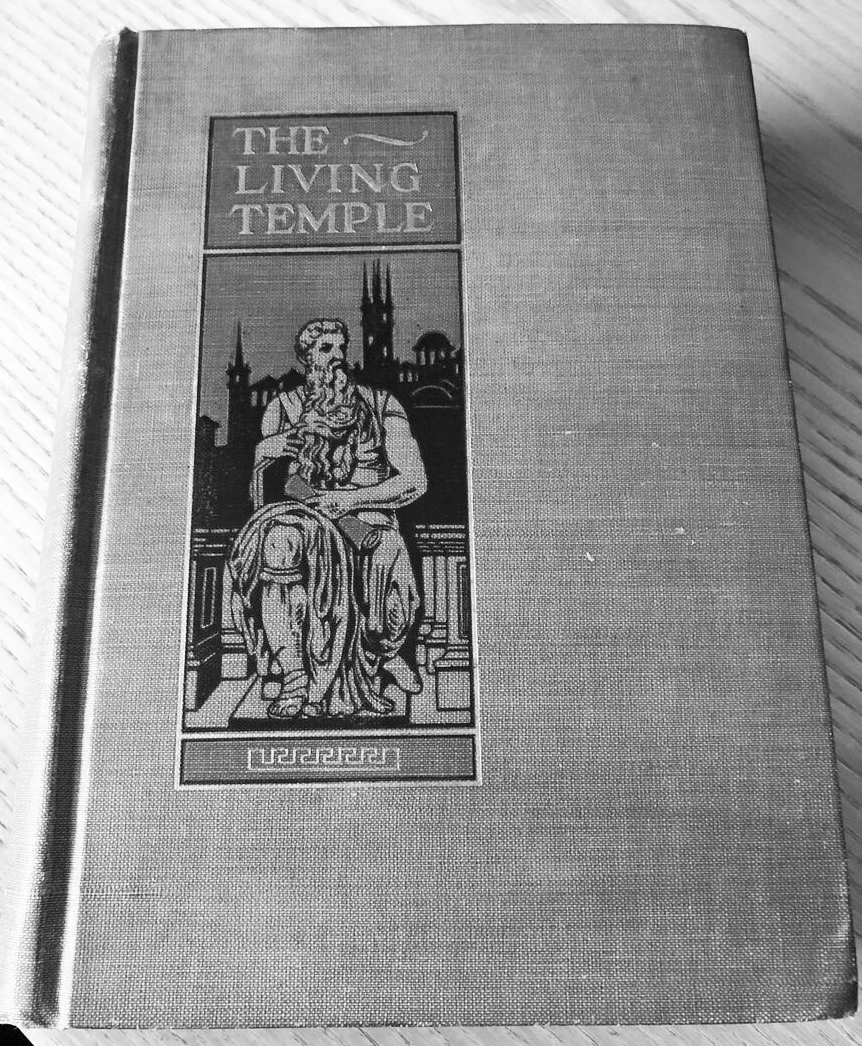
\includegraphics[width=1\linewidth]{images/TLT.jpg}
    \caption*{The Living Temple by Dr. J. H. Kellogg, 1903}
    \label{fig:tlt}
\end{figure}


\begin{figure}[hp]
    \centering
    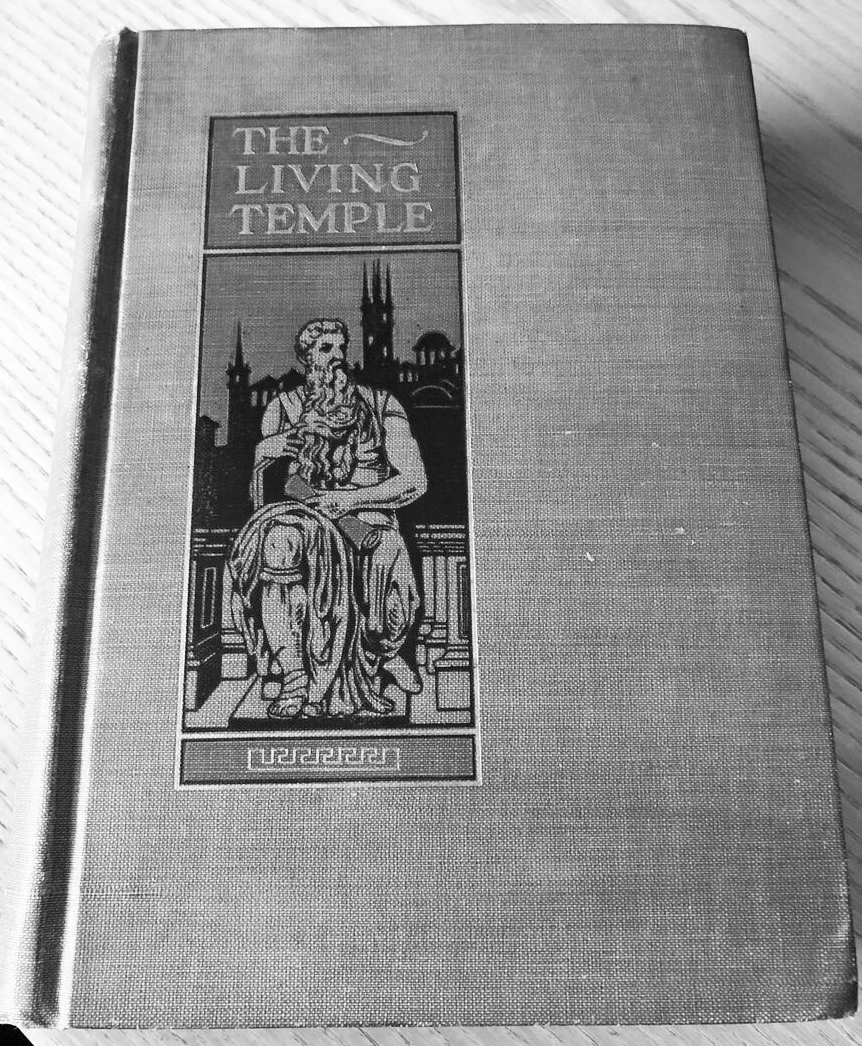
\includegraphics[width=1\linewidth]{images/TLT.jpg}
    \caption*{The Living Temple por el Dr. J. H. Kellogg, 1903}
    \label{fig:tlt}
\end{figure}


Some people find Dr. Kellogg’s understanding of God’s personality resonates with their understanding, yet they are tempted to think that there are other things objectionable with the Living Temple. The following evidence suggests the very opposite. There is a letter from Dr. Kellogg to William C. White, where Dr. Kellogg proposes to \others{cutting out a few leaves} from the three thousand copies of the Living Temple—those very leaves containing the \others{specially objectionable things appear, such as the comment on Isaiah 40} and the sentiments regarding the \emcap{personality of God} (the pages we have read).


Algunas personas encuentran que la comprensión del Dr. Kellogg sobre la personalidad de Dios resuena con su comprensión, sin embargo, están tentados a pensar que hay otras cosas objetables con el Templo Viviente. La siguiente evidencia sugiere lo contrario. Hay una carta del Dr. Kellogg a William C. White, en la que el Dr. Kellogg propone \others{recortar algunas hojas} de los tres mil ejemplares del Templo Viviente—precisamente aquellas hojas que contienen las \others{cosas especialmente objetables, como el comentario sobre Isaías 40} y los sentimientos relativos a la \emcap{personalidad de Dios} (las páginas que hemos leído).


\others{The Sanitarium has on hand, I find, \textbf{two or three thousand books which were sold}, but which have come back since the book was condemned. The question has been raised, what shall be done with these? \textbf{It has occurred to me that perhaps they might be saved \underline{by cutting out a few leaves} in which the \underline{specially objectionable things appear}, such as the \underline{comment on Isaiah 40}, which I borrowed from A.T. Jones, and the page on which the unfortunate heading appears, ‘\underline{The Personality of God},’ and tipping in leaves embodying a clear statement of the Bible view of God as a person presented in Elder Haskell’s article in the ‘Review’ a few weeks ago}. These books would be sold to old patients who are making a great demand for the book for Christmas presents…}[Letter from Dr. J.H. Kellogg to W.C.White; December 6, 1903, Chicago][https://174625.selcdn.ru/ellenwhite/EWhite/17226/17226.pdf]


\others{El Sanitario tiene a mano, según creo, \textbf{dos o tres mil libros que fueron vendidos}, pero que han regresado desde que el libro fue condenado. Se ha planteado la pregunta, ¿qué hacer con ellos? \textbf{Se me ha ocurrido que tal vez podrían salvarse \underline{recortando algunas hojas} en las que aparecen las \underline{cosas especialmente objetables}, como el \underline{comentario sobre Isaías 40}, que tomé prestado de A.T. Jones, y la página en la que aparece el desafortunado título, ‘\underline{La Personalidad de Dios},’ e introduciendo hojas que contengan una clara declaración de la visión bíblica de Dios como persona presentada en el artículo del anciano Haskell en la ‘Review’ hace unas semanas}. Estos libros se venderían a pacientes antiguos que están haciendo una gran demanda del libro para los regalos de Navidad...}[Letter from Dr. J.H. Kellogg to W.C.White; December 6, 1903, Chicago][https://174625.selcdn.ru/ellenwhite/EWhite/17226/17226.pdf]


What is the real issue with the reasoning in the Living Temple? We will study the matter to its very depth; superficially, we clearly see that the issue is the stepping off of the foundation of our faith—the \emcap{Fundamental Principles}—regarding the \emcap{personality of God} and where His presence is.


¿Cuál es el verdadero problema del razonamiento en el Templo Viviente? Estudiaremos el asunto hasta el fondo; superficialmente, vemos claramente que la cuestión es el abandono de los cimientos de nuestra fe—los \emcap{Principios Fundamentales}—con respecto a la \emcap{personalidad de Dios} y dónde está su presencia.


\egw{\textbf{I have been instructed by the heavenly messenger} that \textbf{some of the reasoning} in the book, ‘Living Temple’, is unsound and that \textbf{this reasoning would lead astray} the minds of those who are not thoroughly established on \textbf{the foundation principles} of present truth. \textbf{It introduces that which is naught but speculation} in \textbf{regard to the personality of God and where His presence is}.}[SpTB02 51.3; 1904][https://egwwritings.org/read?panels=p417.262]


\egw{\textbf{He sido instruida por el mensajero celestial} que \textbf{algunos de los razonamientos} en el libro ‘Templo Viviente’, no son sólidos y que \textbf{este razonamiento desviaría} las mentes de aquellos que no están completamente establecidos en \textbf{los principios fundamentales} de la verdad presente. \textbf{Introduce lo que no es más que especulación} con \textbf{respecto a la personalidad de Dios y dónde está su presencia}.}[SpTB02 51.3; 1904][https://egwwritings.org/read?panels=p417.262]


Dr. Kellogg introduced the thought \egwinline{which is naught but speculation in regard to the personality of God}, by which he stepped off of the foundation of our faith—the \emcap{Fundamental Principles}. Discordance between Dr. Kellogg’s teaching and the \emcap{Fundamental Principles} is in the first statement of the principles where we are taught that\others{That there is \textbf{one God}, \textbf{a personal, spiritual \underline{being}}, \textbf{the creator of all things}, ... and \textbf{everywhere present by his representative, the Holy Spirit}. Ps. 139:7.}


El Dr. Kellogg introdujo el pensamiento \egwinline{que no es más que especulación con respecto a la personalidad de Dios}, con lo cual se apartó del fundamento de nuestra fe—los \emcap{Principios Fundamentales}. La discordancia entre la enseñanza del Dr. Kellogg y los \emcap{Principios Fundamentales} está en la primera declaración de los principios donde se nos enseña que\others{Que hay \textbf{un Dios}, \textbf{un ser personal y espiritual \underline{ser}}, \textbf{el creador de todas las cosas}, ... y \textbf{presente en todas partes por su representante, el Espíritu Santo}. Sal. 139:7.}


Sister White directly warned us of the sentiments expressed in the Living Temple regarding the \emcap{personality of God}. They are not in harmony with the first point of the \emcap{Fundamental Principles}, which were part of the foundation of our faith.


La hermana White nos advirtió directamente de los sentimientos expresados en el Templo Viviente respecto a la \emcap{personalidad de Dios}. No están en armonía con el primer punto de los \emcap{Principios Fundamentales}, que formaban parte de la base de nuestra fe.


\egw{\textbf{I have had to write much concerning the strange doctrines and theories expressed in Living Temple. \underline{Were these theories accepted by our people, the strong pillars of our faith and the truths that have made Seventh-day Adventists what they are would be swept away}. I have had to show the fallacy of these doctrines, presenting them \underline{as a species of last-day heresy}. We are told by the Word of God that just such teaching \underline{will be brought in at this time}.}}[Lt250-1903.2; 1903][https://egwwritings.org/read?panels=p9337.8]


\egw{\textbf{He tenido que escribir mucho sobre las extrañas doctrinas y teorías expresadas en el Templo Viviente. \underline{Si estas teorías fueran aceptadas por nuestro pueblo, los fuertes pilares de nuestra fe y las verdades que han hecho de los Adventistas del Séptimo Día lo que son, serían barridos}. He tenido que mostrar la falacia de estas doctrinas, presentándolas \underline{como una especie de herejía de los últimos días}. La Palabra de Dios nos dice que justamente esa enseñanza \underline{será introducida en este tiempo}.}}[Lt250-1903.2; 1903][https://egwwritings.org/read?panels=p9337.8]


Today we witness the widespread acceptance of Kellogg’s theories regarding the \emcap{personality of God}. The fact that the first point of the \emcap{Fundamental Principles} is no longer present in our beliefs proves that Kellogg’s theories regarding the \emcap{personality of God} have had an influence in shaping our beliefs.


Hoy somos testigos de la aceptación generalizada de las teorías de Kellogg con respecto a la \emcap{personalidad de Dios}. El hecho de que el primer punto de los \emcap{Principios Fundamentales} ya no esté presente en nuestras creencias demuestra que las teorías de Kellogg con respecto a la \emcap{personalidad de Dios} han tenido una influencia en la formación de nuestras creencias.


\egw{One and another come to me, asking me to \textbf{explain the positions taken in “Living Temple.”} I reply, “They are unexplainable.” \textbf{The sentiments expressed do not give a true knowledge of God.} \textbf{All through the book are passages of scripture}. \textbf{These scriptures are brought in in such a way \underline{that error is made to appear as truth}}. \textbf{Erroneous theories are presented in so pleasing a way that unless care is taken, many will be misled}.}[SpTB02 52.1; 1904][https://egwwritings.org/read?panels=p417.265]


\egw{Uno y otro vienen a mí, pidiéndome que \textbf{explique las posiciones adoptadas en “Templo Viviente.”} Yo respondo, “Son inexplicables.” \textbf{Los sentimientos expresados no dan un verdadero conocimiento de Dios.} \textbf{A lo largo del libro hay pasajes de las escrituras}. \textbf{Estas escrituras se presentan de tal manera \underline{que el error se hace aparecer como verdad}}. \textbf{Las teorías erróneas se presentan de manera tan agradable que, a menos que se tenga cuidado, muchos serán engañados}.}[SpTB02 52.1; 1904][https://egwwritings.org/read?panels=p417.265]


The error is being made to appear as truth, and many are misled.


El error se hace aparecer como verdad, y muchos son engañados.


It is worth emphasizing, for some careless reader, that the real issue of Dr. Kellogg, and his book “\textit{Living Temple}”, is not the Trinity but the small step he took off of the \emcap{Fundamental Principles}. In order to understand the real issue of his book, it would be wrong to focus on its overlapping sentiments with the Trinity doctrine. Rather, we should focus on the point that constituted this small step he made; and this includes having a deep understanding of the \emcap{fundamental principles} just as our pioneers had. Who better to ask than the Adventist pioneers themselves?


Vale la pena enfatizar, para algún lector descuidado, que el verdadero asunto del Dr. Kellogg, y su libro “\textit{Living Temple}”, no es la Trinidad sino el pequeño paso que dio de los \emcap{Principios Fundamentales}. Para entender el verdadero tema de su libro, sería un error centrarse en sus sentimientos superpuestos con la doctrina trinitaria. Más bien, deberíamos centrarnos en el punto que constituyó este pequeño paso que dio; y esto incluye tener una comprensión profunda de los \emcap{principios fundamentales}, tal como la tuvieron nuestros pioneros. ¿Quién mejor para preguntar que los propios pioneros adventistas?


% Constructive Criticism

\begin{titledpoem}
    
    \stanza{
        A personal God in heaven sits enthroned, \\
        This truth in our Principles firmly zoned. \\
        Present everywhere by Spirit's might, \\
        This foundation stood as our guiding light.
    }

    \stanza{
        Then came words that seemed so wise and deep, \\
        A subtle shift that made the faithful weep. \\
        "God's form beyond all human thought," they claimed, \\
        A mystery too vast to be contained or named.
    }

    \stanza{
        "Discussions of God's form," the Temple said, \\
        "Are futile paths where idols lie ahead." \\
        Yet this philosophy so smoothly spun, \\
        Was the very snare by which souls were won.
    }

    \stanza{
        The error dressed as truth appeared so fair, \\
        As scripture twisted in a clever snare. \\
        One small step from the Principles we held, \\
        One giant leap by which our faith was felled.
    }

    \stanza{
        Beware the mind that thinks itself too wise, \\
        To see deception veiled in truth's disguise. \\
        God is personal, definite, and real, \\
        This is the truth the Temple would conceal. 
    }
\end{titledpoem}


% Constructive Criticism

\begin{titledpoem}
    
    \stanza{
        A personal God in heaven sits enthroned, \\
        This truth in our Principles firmly zoned. \\
        Present everywhere by Spirit's might, \\
        This foundation stood as our guiding light.
    }

    \stanza{
        Then came words that seemed so wise and deep, \\
        A subtle shift that made the faithful weep. \\
        "God's form beyond all human thought," they claimed, \\
        A mystery too vast to be contained or named.
    }

    \stanza{
        "Discussions of God's form," the Temple said, \\
        "Are futile paths where idols lie ahead." \\
        Yet this philosophy so smoothly spun, \\
        Was the very snare by which souls were won.
    }

    \stanza{
        The error dressed as truth appeared so fair, \\
        As scripture twisted in a clever snare. \\
        One small step from the Principles we held, \\
        One giant leap by which our faith was felled.
    }

    \stanza{
        Beware the mind that thinks itself too wise, \\
        To see deception veiled in truth's disguise. \\
        God is personal, definite, and real, \\
        This is the truth the Temple would conceal. 
    }
\end{titledpoem}
